% 图 6.5 NH3 分子两个取向 (a)(b)、双阱势能 (c)、第一激发态 phi1 (d)、基态 phi0 (e)
\documentclass[tikz,border=5pt]{standalone}
\usetikzlibrary{arrows.meta}
\usepackage{amsmath}
\usepackage{bm}
\usepackage{fontspec}
\setmainfont{Times New Roman}
\begin{document}
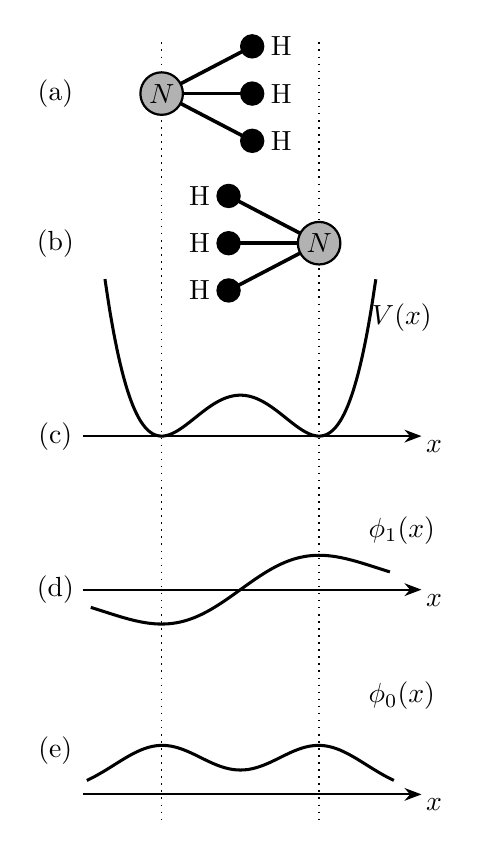
\begin{tikzpicture}[line width=0.8pt,>=Stealth]
% dotted guide lines x=0 (left well) and x=2 (right well), through all panels
\draw[dotted,line width=0.55] (0,9.55) -- (0,-0.35);
\draw[dotted,line width=0.55] (2,9.55) -- (2,-0.35);
% ---- (a) N on the left site ----
\node at (-1.35,8.9) {(a)};
\draw[line width=1.3pt] (0,8.9) -- (1.15,9.5);
\draw[line width=1.3pt] (0,8.9) -- (1.15,8.9);
\draw[line width=1.3pt] (0,8.9) -- (1.15,8.3);
\filldraw[fill=gray!60] (0,8.9) circle (0.27) node {$N$};
\foreach \y in {9.5,8.9,8.3}{
  \fill (1.15,\y) circle (0.155);
  \node at (1.52,\y) {$\mathrm{H}$};
}
% ---- (b) N on the right site ----
\node at (-1.35,7.0) {(b)};
\draw[line width=1.3pt] (2,7.0) -- (0.85,7.6);
\draw[line width=1.3pt] (2,7.0) -- (0.85,7.0);
\draw[line width=1.3pt] (2,7.0) -- (0.85,6.4);
\filldraw[fill=gray!60] (2,7.0) circle (0.27) node {$N$};
\foreach \y in {7.6,7.0,6.4}{
  \fill (0.85,\y) circle (0.155);
  \node at (0.48,\y) {$\mathrm{H}$};
}
% ---- (c) double-well potential ----
\node at (-1.35,4.55) {(c)};
\draw[->,line width=0.7pt] (-1.0,4.55) -- (3.3,4.55)
  node[below right=-2pt] {$x$};
\draw[line width=1.1pt,domain=-0.72:2.72,samples=61,smooth]
  plot ({\x},{4.55+0.52*((\x-1)*(\x-1)-1)*((\x-1)*(\x-1)-1)});
\node at (3.05,6.05) {$V(x)$};
% ---- (d) first excited state phi1 ----
\node at (-1.35,2.6) {(d)};
\draw[->,line width=0.7pt] (-1.0,2.6) -- (3.3,2.6)
  node[below right=-2pt] {$x$};
\draw[line width=1.1pt,domain=-0.9:2.9,samples=81,smooth]
  plot ({\x},{2.6+0.72*(\x-1)*exp(-(\x-1)*(\x-1)/2)});
\node at (3.05,3.35) {$\phi_1(x)$};
% ---- (e) ground state phi0 ----
\node at (-1.35,0.55) {(e)};
\draw[->,line width=0.7pt] (-1.0,0.0) -- (3.3,0.0)
  node[below right=-2pt] {$x$};
\draw[line width=1.1pt,domain=-0.95:2.95,samples=81,smooth]
  plot ({\x},{0.62*(exp(-\x*\x/0.72)+exp(-(\x-2)*(\x-2)/0.72))});
\node at (3.05,1.25) {$\phi_0(x)$};
\end{tikzpicture}
\end{document}
